\chapter{Multilayer Perceptron}
\label{chap:MLP}

In questo capitolo e nel Capitolo \ref{chap:CNN} sono stati replicati, in piccola scala, i risultati ottenuti nel paper di ResNet \cite{resnet}. Si è voluto quindi dimostrare che andare più in profondità non vuol dire in ogni caso aumentare le prestazioni del modello. Inoltre si è poi notato come aggiungendo le residual connection si ottengono risultati migliori anche per le reti più profonde.

Per svolgere il compito di classificazione è stato usato il dataset MNIST, presentato nella Sezione \ref{sec:MNIST}.

\subsection{Scelte}
Ho deciso di non valutare utilizzare un validation set, ma di basarmi solo sul train e test set. Il mio obiettivo non era infatti quello di valutare le prestazioni di un modello in relazione a più iperparametri oppure di migliorare un dato modello per ottenere performance sempre migliori, ma solo di capire se e a quale profondità la rete smetteva di imparare. Un validation set infatti è utile per non includere nell'addestramento informazioni su dati che saranno poi usati in fase di testing; in questo caso infatti non riusciremo a capire quanto bene il modello generalizza.

\myskip

Nel caso del MLP senza residual block stati usati 4 modelli, con un numero crescente di layer (progetti di tipo \texttt{nn.Linear}): 4, 13, 23 e 33.
I modelli testati con le residual connection sono invece 5: sono stati aggiunti due modelli molto profondi per valutare le prestazioni su un numero di layer (molto) elevato.

In tutti gli esperimenti il numero all'interno dei nomi che vedremo nei grafici è relativo al numero di layer del modello.

%%%%%%%%%%%%%%%%%%%%%%%%%%%%%%%%%%%%%%%%%%%%%%%%%%%%
\section{Analisi senza residual connection}
Partiamo dall'osservare la Figura \ref{fig:MLPlowdeep}, relativa alla loss e all'accuracy delle reti con 4, 13 e 23 layer lineari. Si può osservare come le performance del modello siano inversamente proporzionali alla sua profondità. Il modello più profondo infatti ha ottenuto i risultati peggiori sia nell'accuracy sul test set che nella loss sul train set. Già questo è un primo risultato che verifica la tesi. Inoltre se osserviamo bene MLP\_23 possiamo vedere che nelle prime epoche è nettamente peggiore rispetto agli altri.

\begin{figure}[htbp]
    \centering
    \begin{subfigure}{0.45\textwidth}
        \centering
        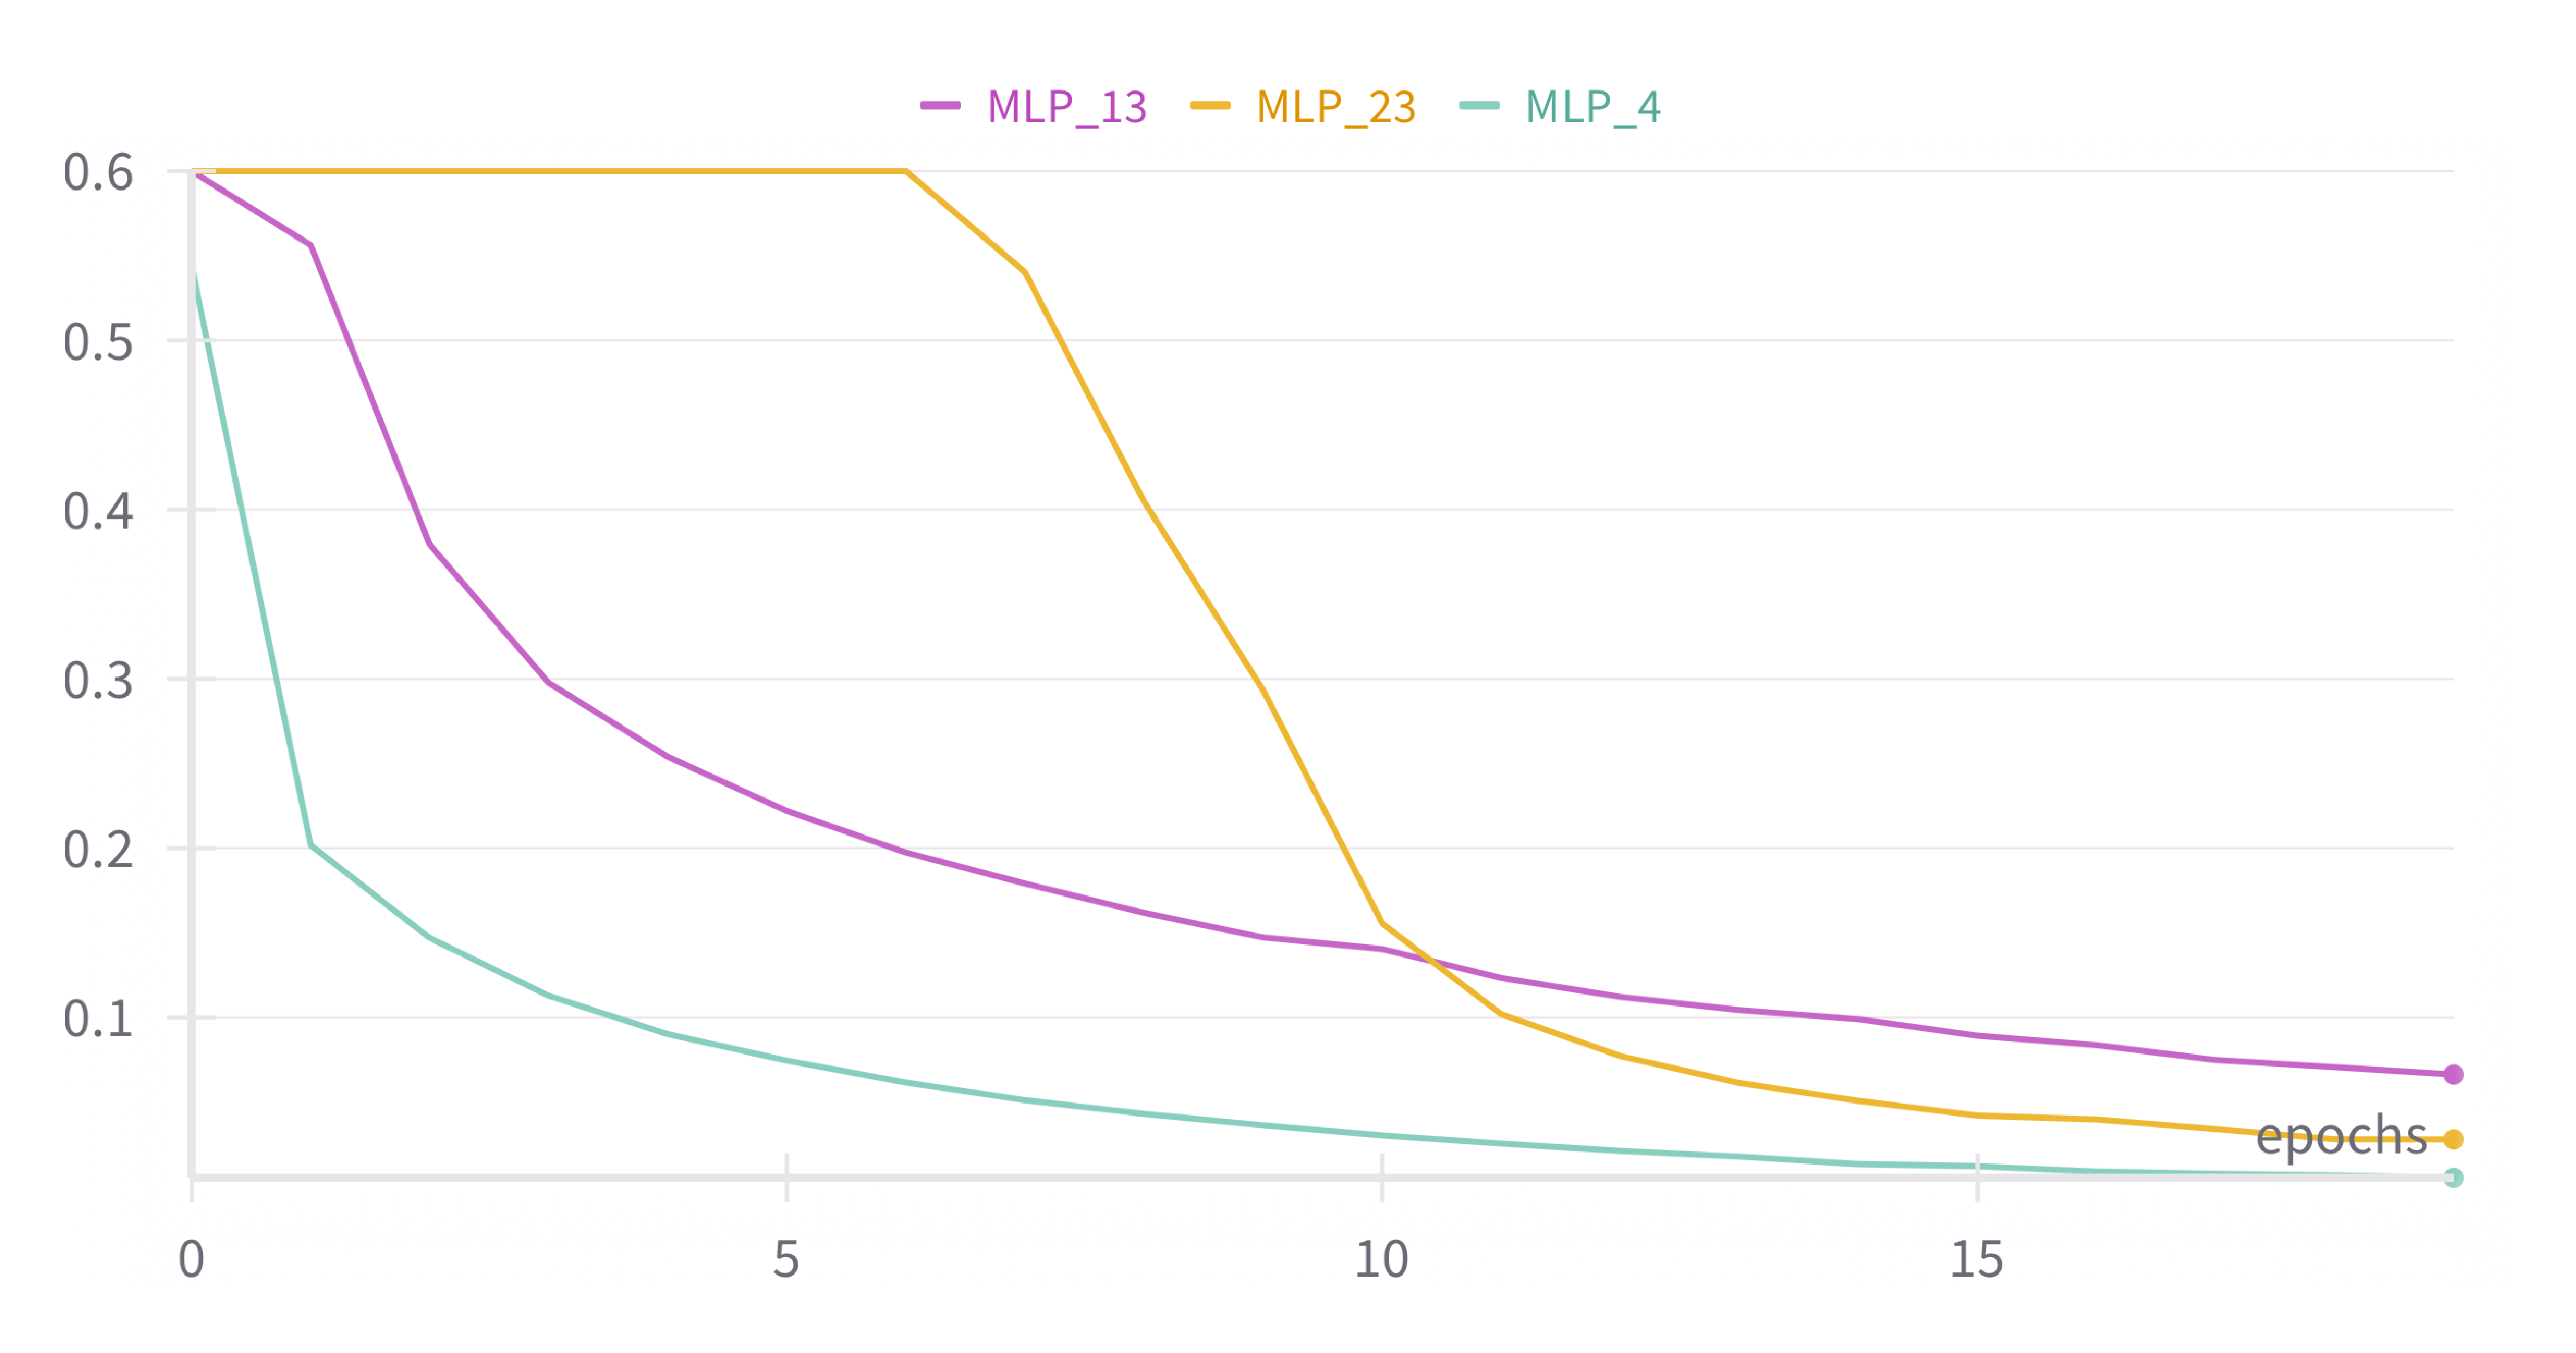
\includegraphics[width=\textwidth]{immages/3-MLP/loss ok.pdf}
        \caption{Loss}
    \end{subfigure}
    \hfill
    \begin{subfigure}{0.45\textwidth}
        \centering
        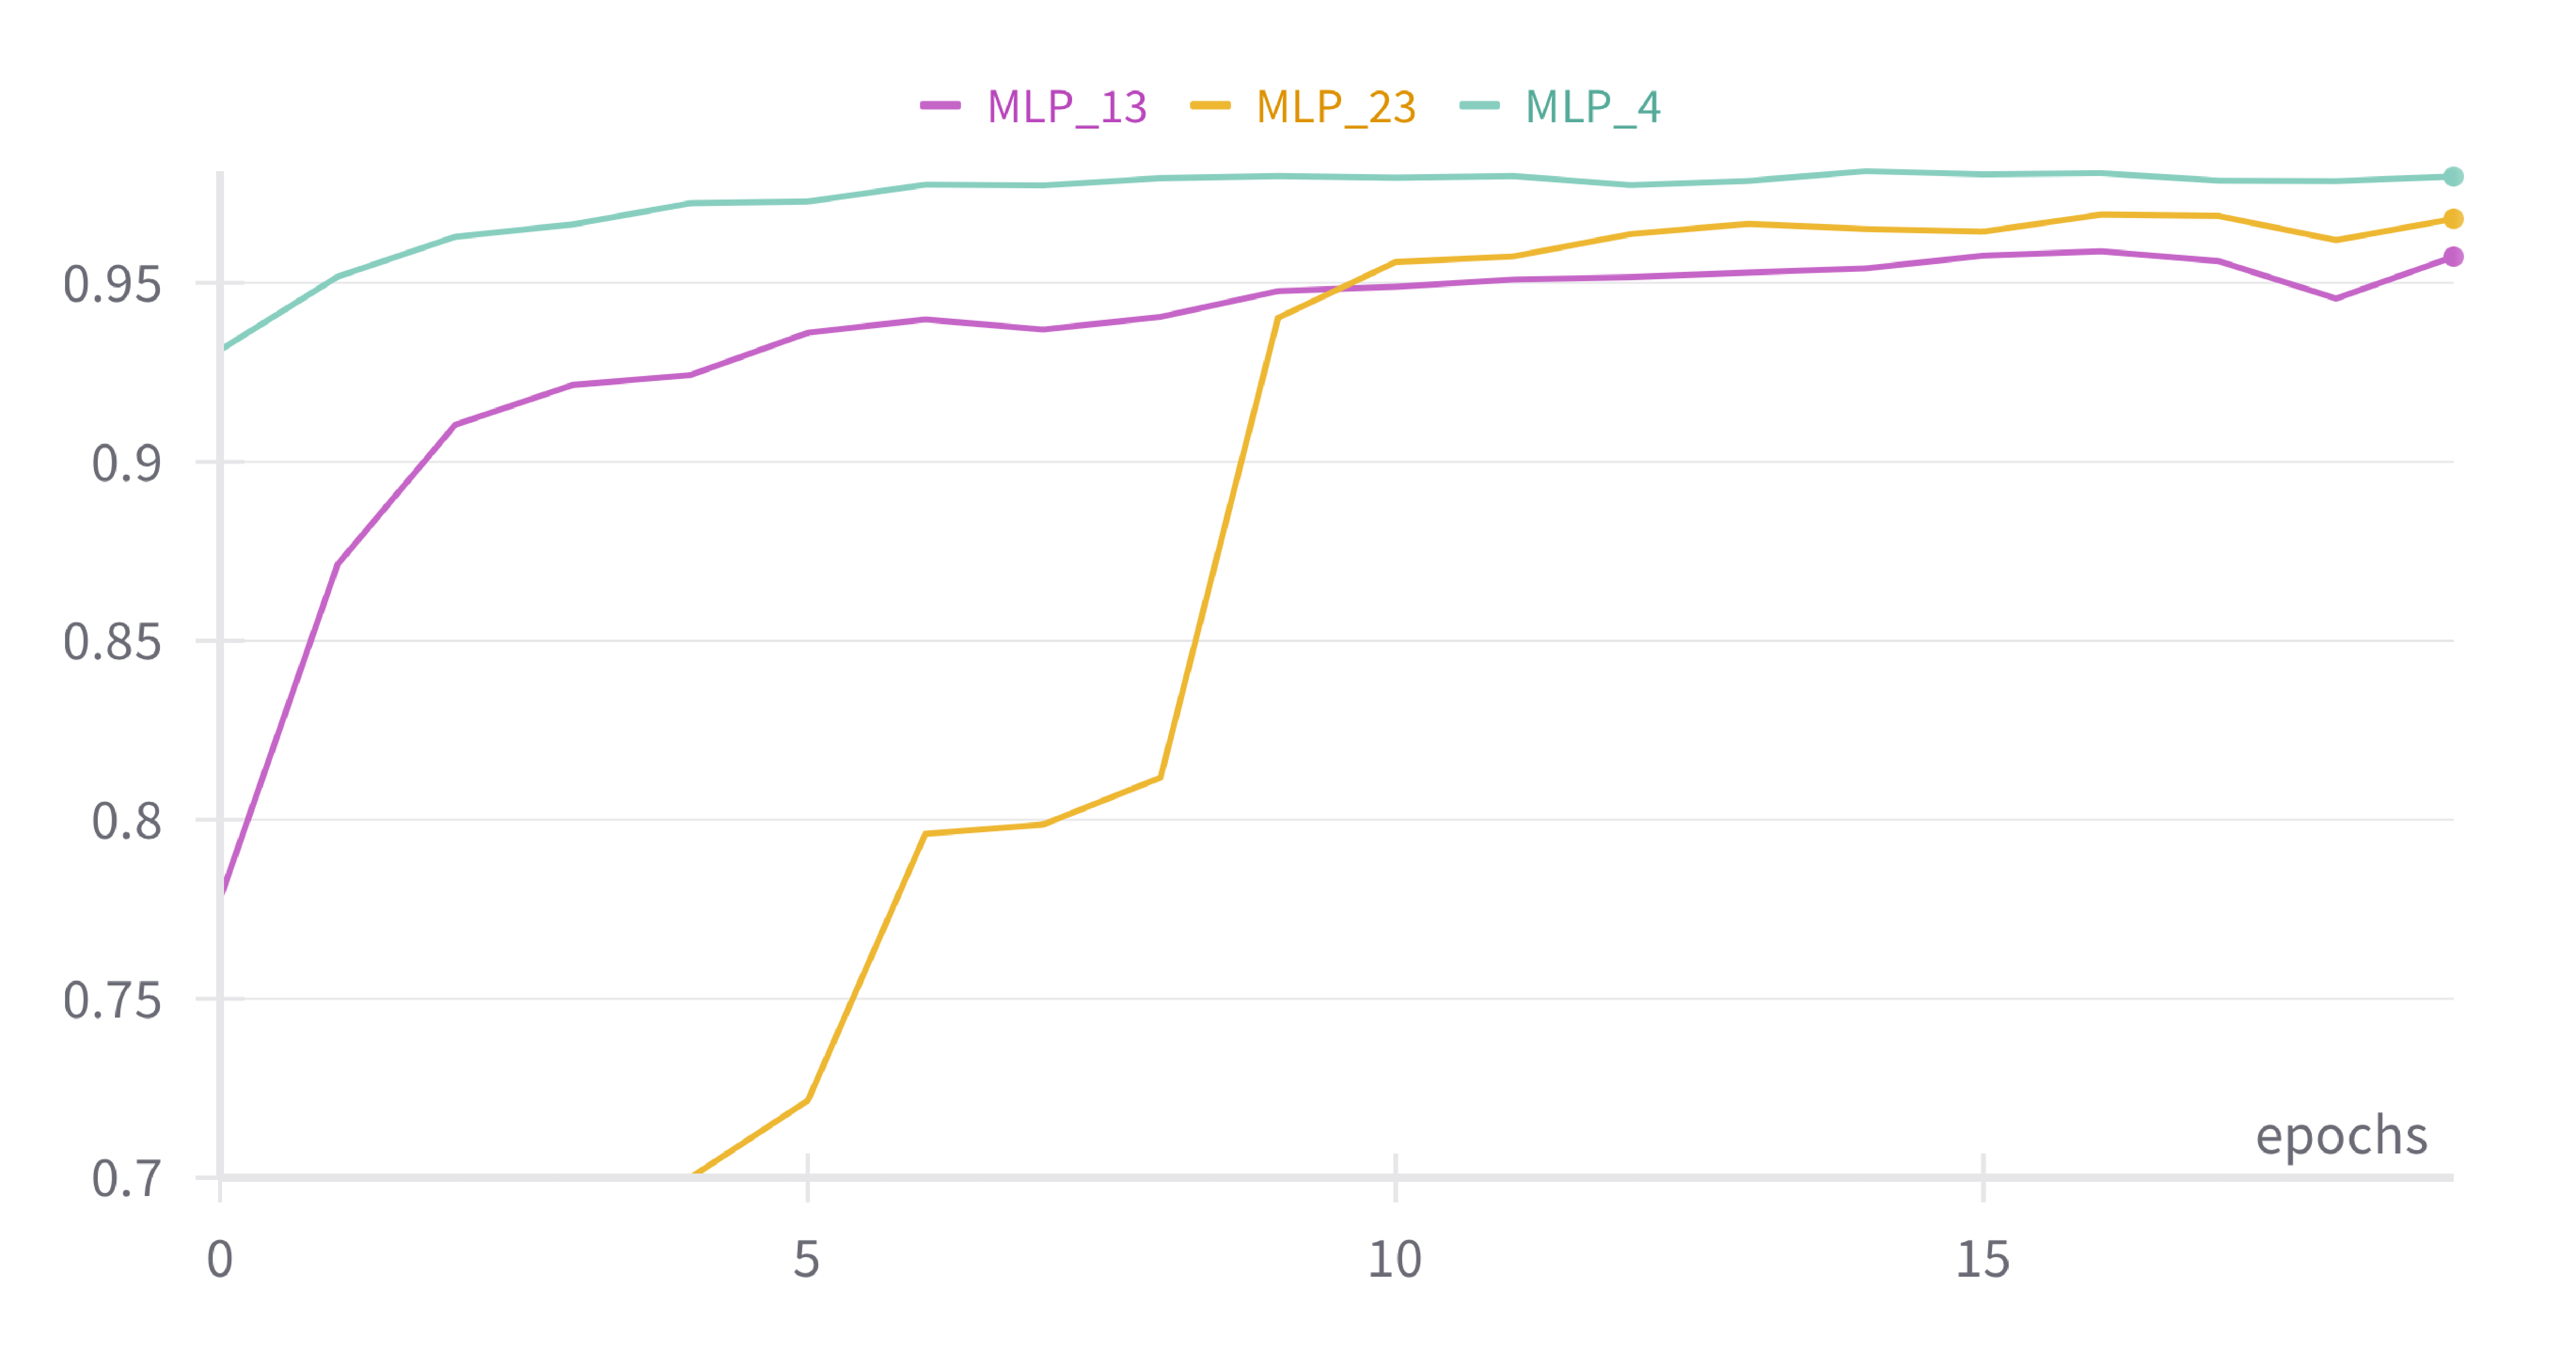
\includegraphics[width=\textwidth]{immages/3-MLP/acc ok.pdf}
        \caption{Accuracy}
    \end{subfigure}
    \caption{Loss e Accuracy MLP\_4, MLP\_13 e MLP\_23.}
    \label{fig:MLPlowdeep}
\end{figure}

\myskip

Analizziamo ora i grafici in Figura \ref{fig:MLPdeepest} relativi a MLP\_33, il multilayer perceptron più profondo testato.
È chiaro come la rete non stia imparando nulla. La loss è molto alta (circa 2,3) e non riesce minimamente a convergere verso l'ottimo; l'accuracy è pari a 0,1, che equivale a lanciare un dado con 10 facce.

\begin{figure}[htbp]
    \centering
    \begin{subfigure}{0.45\textwidth}
        \centering
        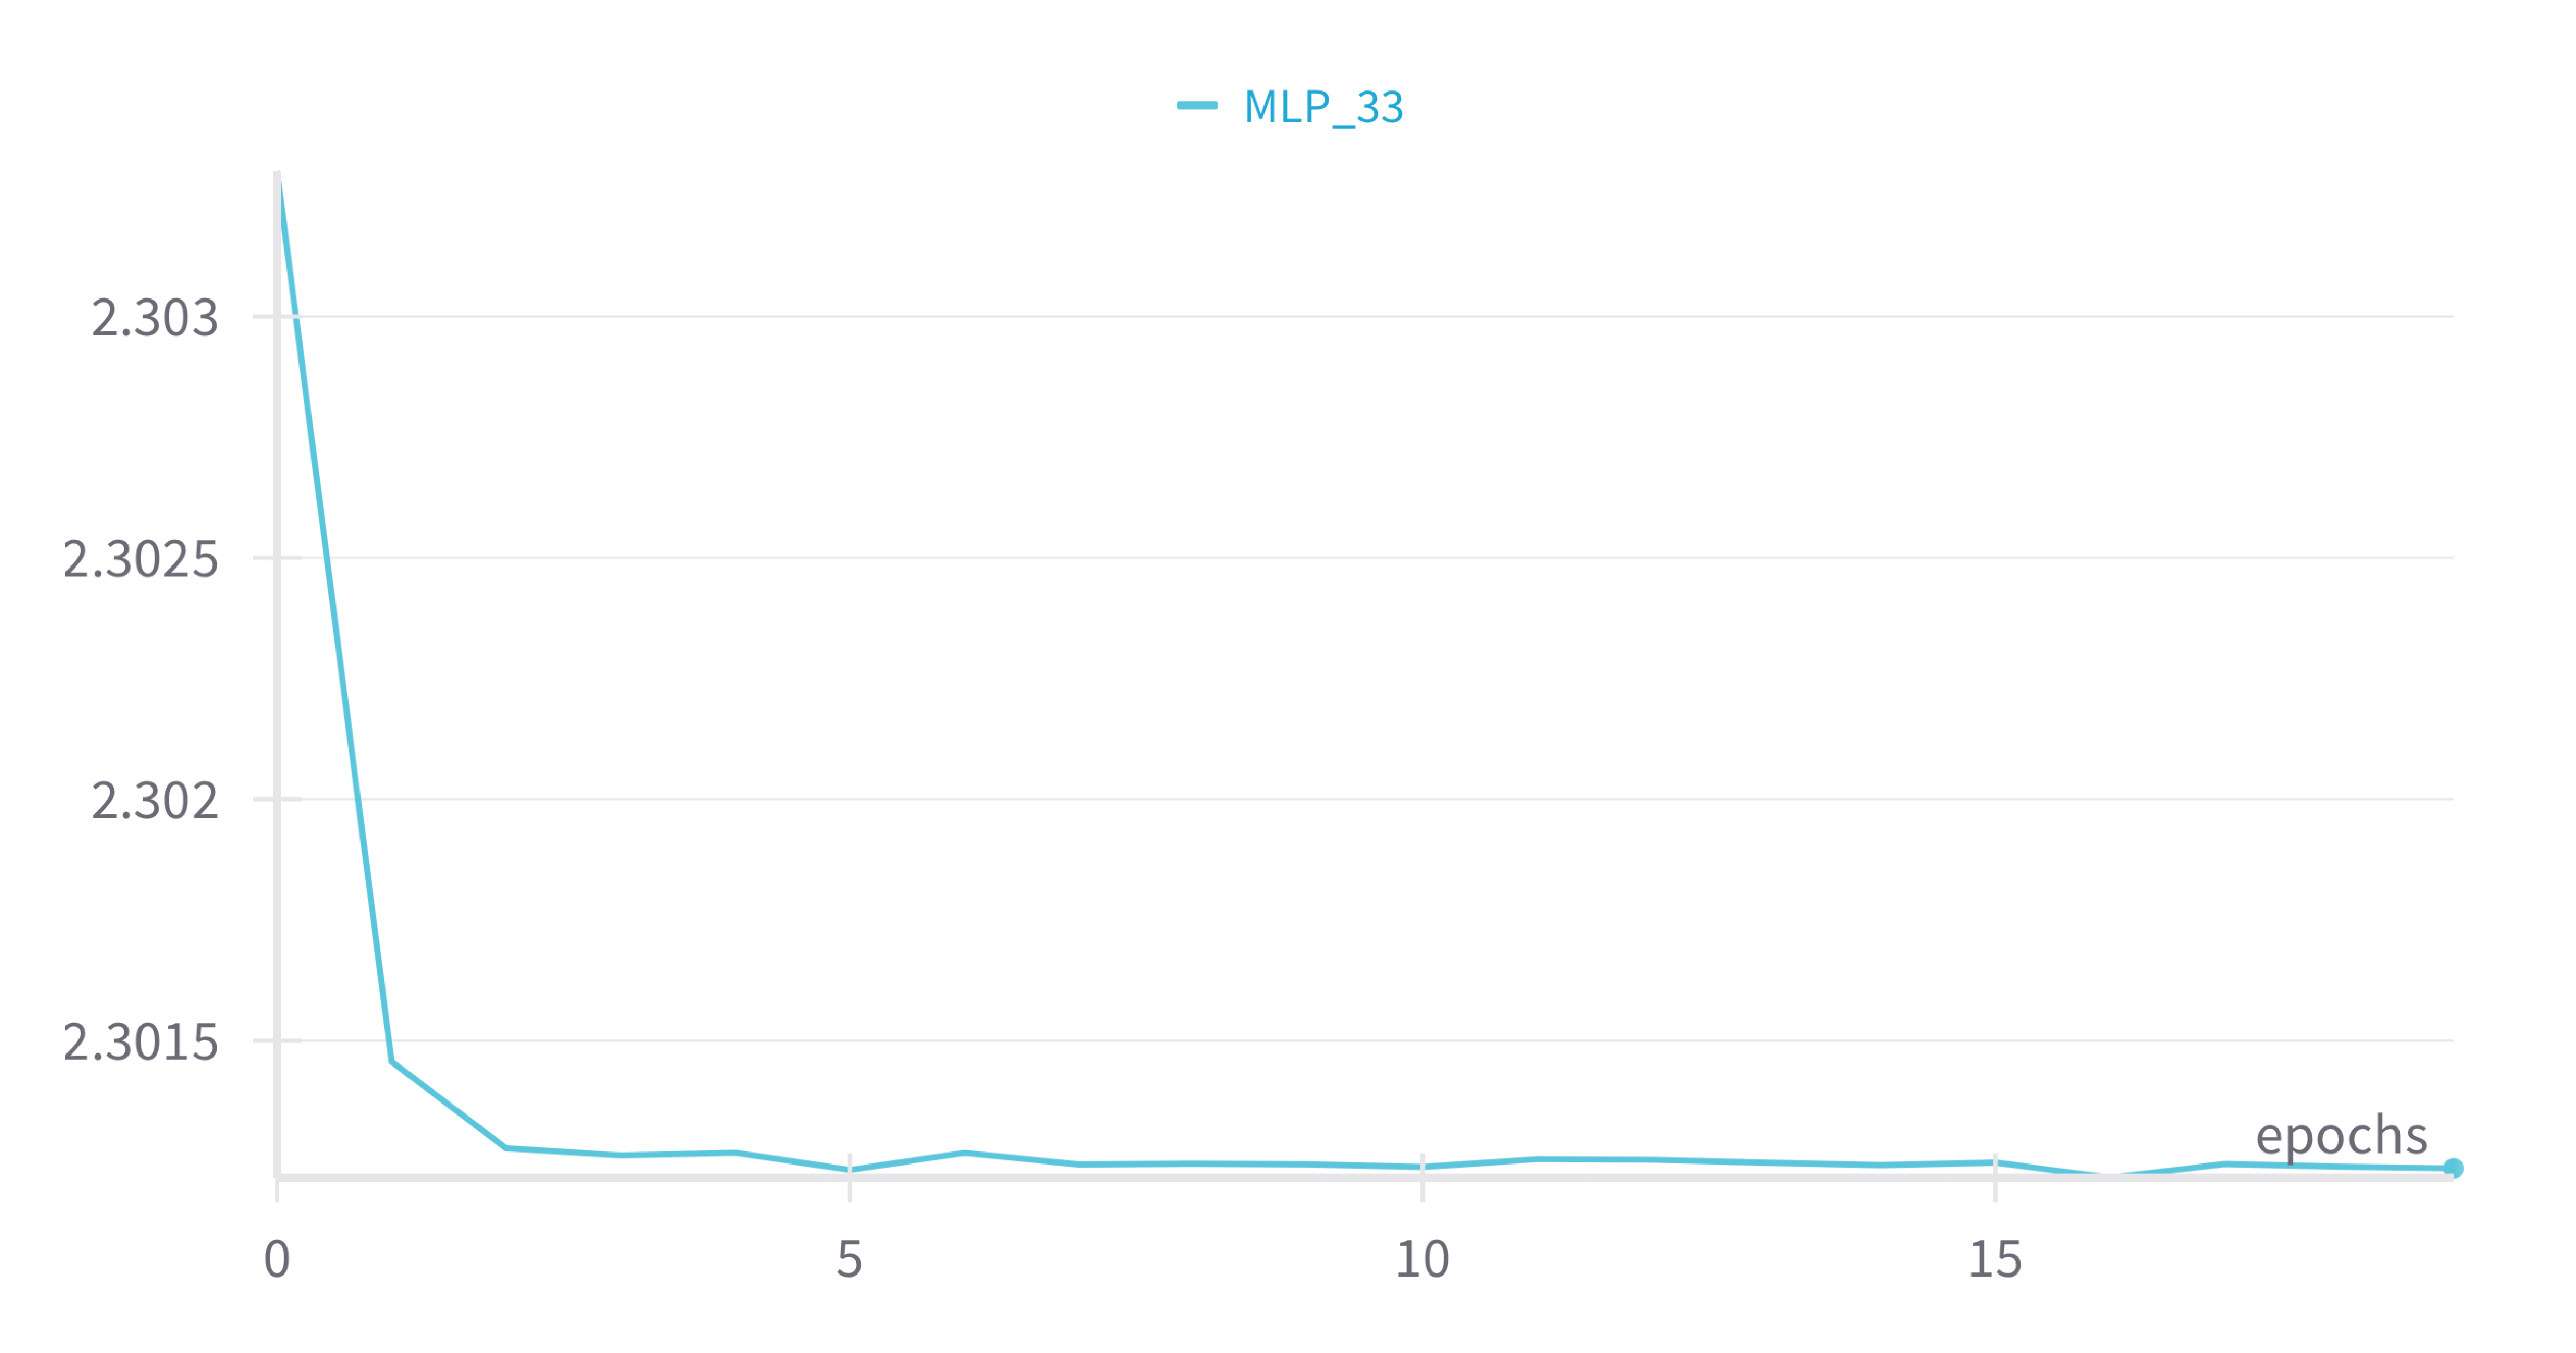
\includegraphics[width=\textwidth]{immages/3-MLP/loss ko.pdf}
        \caption{Loss}
    \end{subfigure}
    \hfill
    \begin{subfigure}{0.45\textwidth}
        \centering
        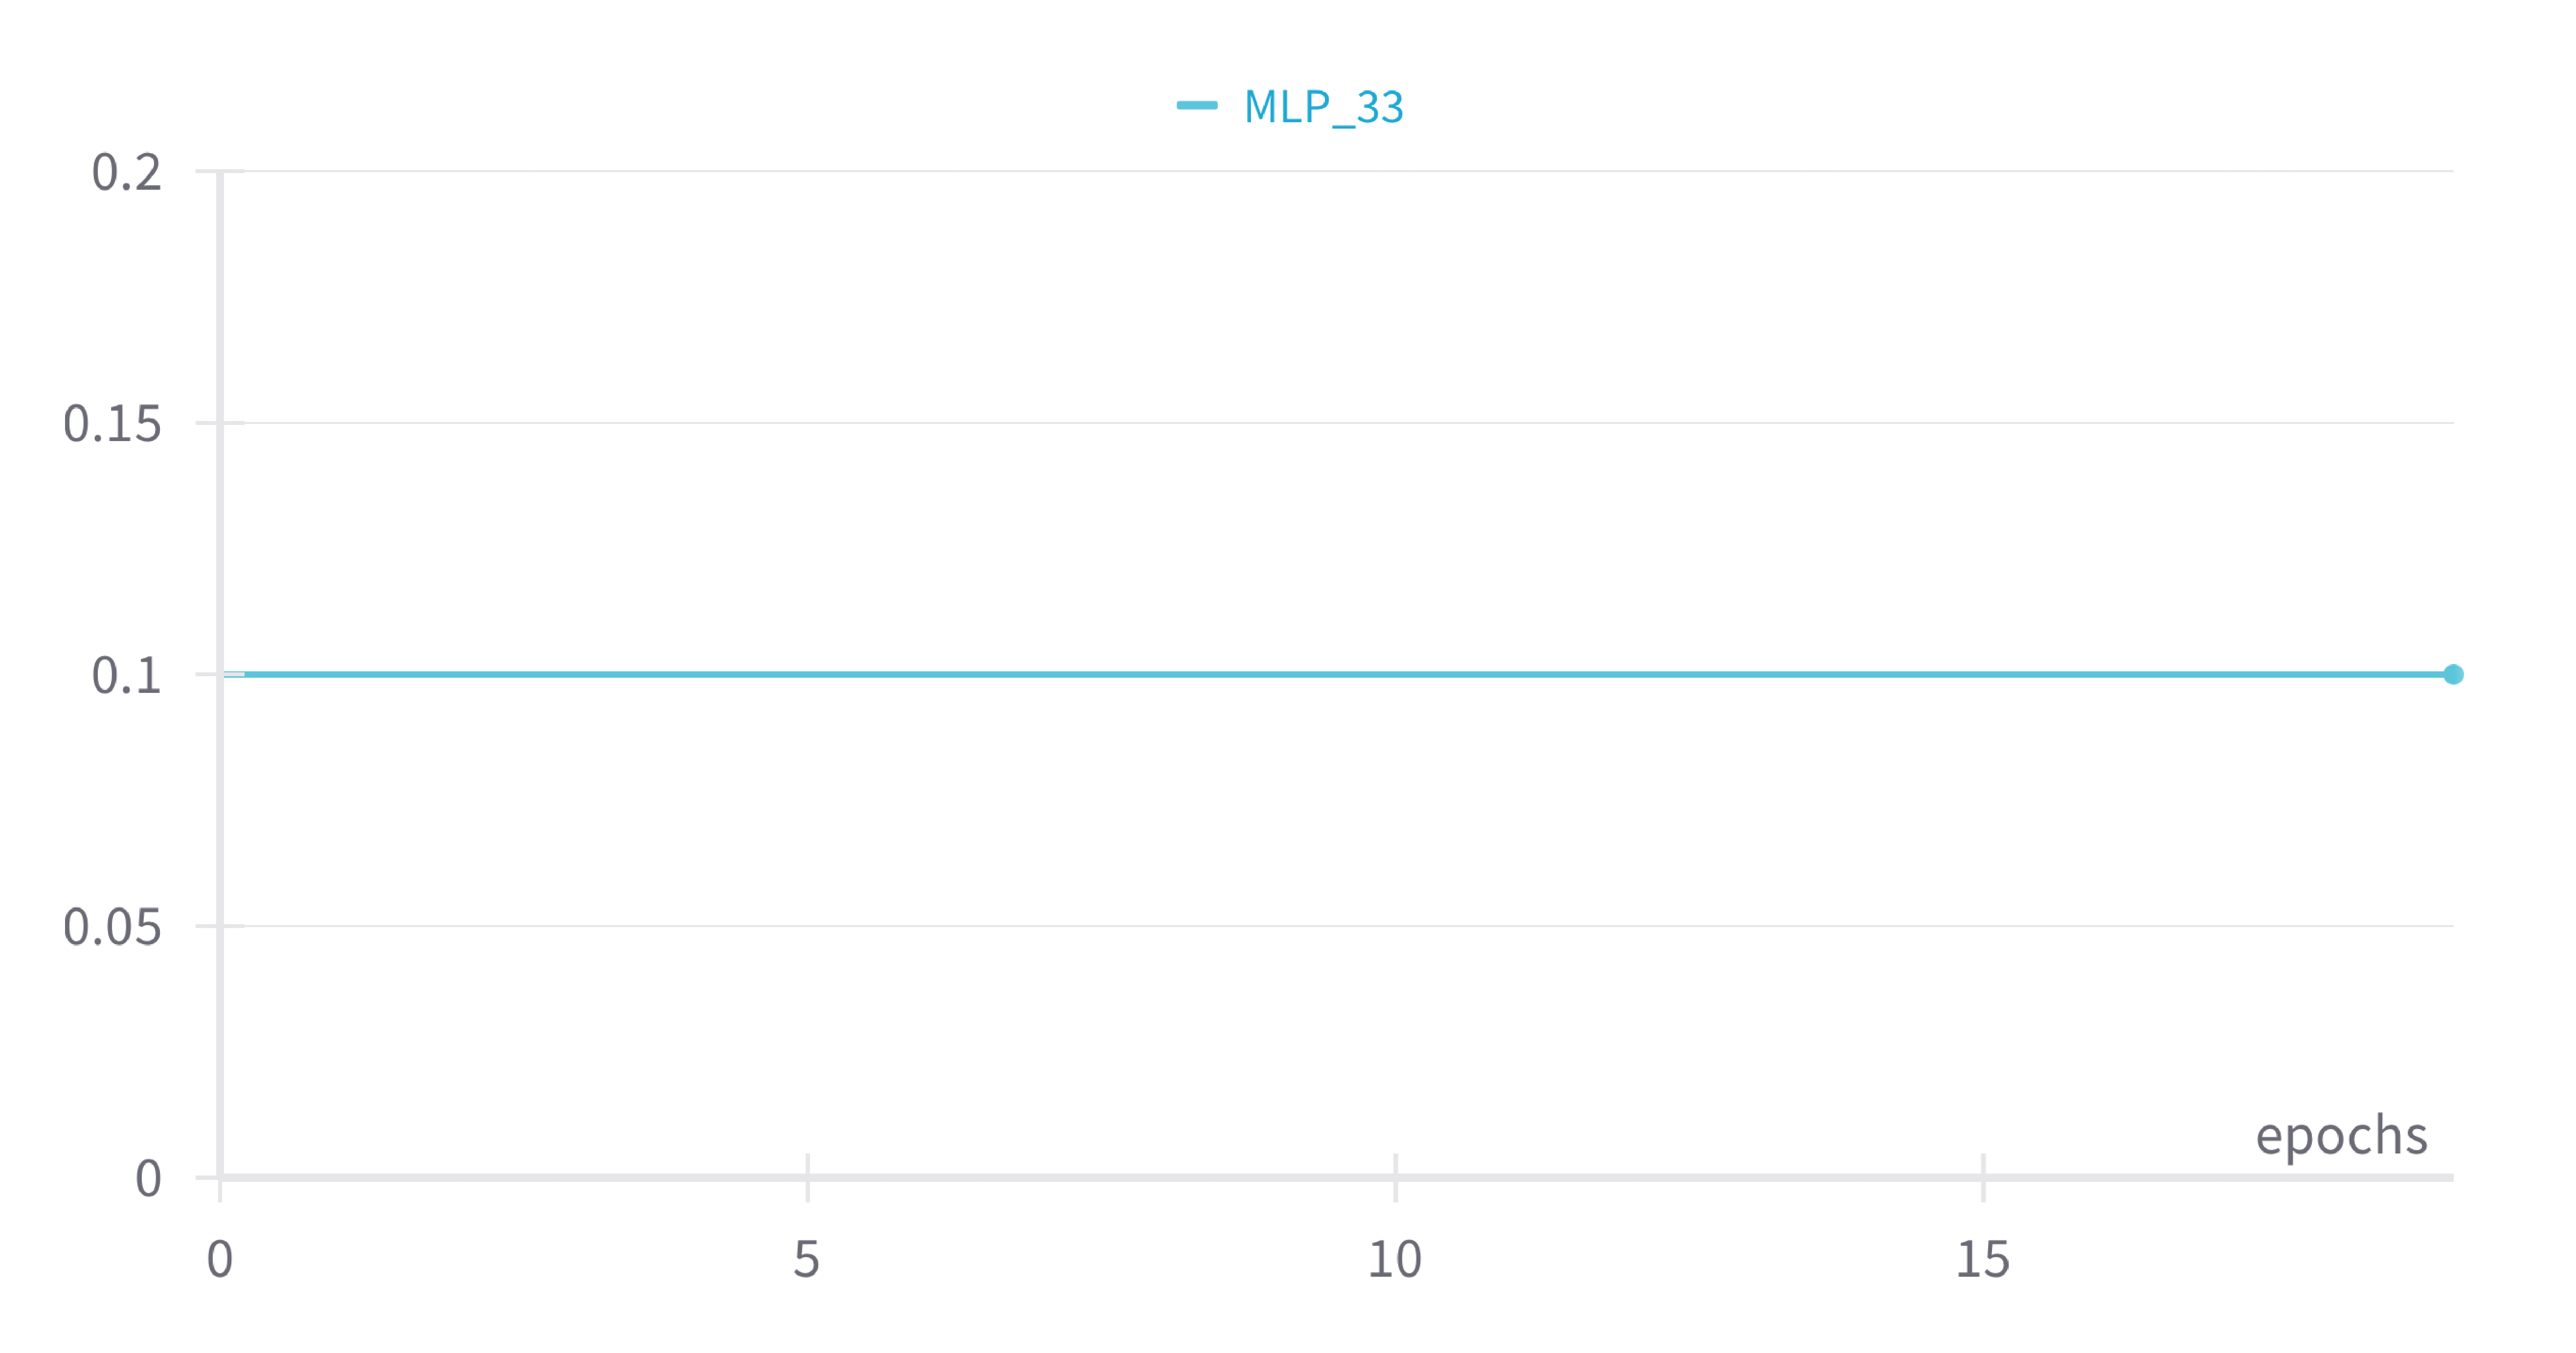
\includegraphics[width=\textwidth]{immages/3-MLP/acc ko.pdf}
        \caption{Accuracy}
    \end{subfigure}
    \caption{Loss e Accuracy MLP\_33.}
    \label{fig:MLPdeepest}
\end{figure}

\myskip

Un'analisi interessante è quella relativa alle norme dei gradienti delle varie reti. Quello che ho fatto è stato sommare per ogni parametro la norma del suo gradiente alla fine di ogni epoca.

In Figura \ref{fig:gradok} si osservano i gradienti dei modelli meno profondi, quelli con 4, 13 e 23 layer. Si può notare come le prestazioni siano inversamente proporzionali alla norma; probabilmente dovrebbero essere fatti altri esperimenti e non si può dire che il risultato sia definitivo, però di sicuro è qualcosa di interessante. Se invece osserviamo la Figura \ref{fig:gradko} vediamo il risultato sul modello con 33 layer; in questo caso è chiaro che i risultati relativi all'accuracy nell'esperimento di questo modello sono dovuti al problema del vanishing gradient.

\begin{figure}[htbp]
    \centering
    \begin{subfigure}{0.45\textwidth}
        \centering
        \includegraphics[width=\textwidth]{immages/3-MLP/grad ok.pdf}
        \caption{Modelli meno profondi}
        \label{fig:gradok}
    \end{subfigure}
    \hfill
    \begin{subfigure}{0.45\textwidth}
        \centering
        \includegraphics[width=\textwidth]{immages/3-MLP/grad ko.pdf}
        \caption{Modello profondo}
        \label{fig:gradko}
    \end{subfigure}
    \caption{Analisi sulla somma delle norme dei parametri.}
\end{figure}

%%%%%%%%%%%%%%%%%%%%%%%%%%%%%%%%%%%%%%%%%%%%%%%%%%%%
\section{Analisi con residual connection}
L'utilizzo delle residual connection, come si può osservare dai risultati in Figura \ref{fig:MLPres}, aiutano la rete a non perdere totalmente le prestazioni. Anche con moltissimi (forse troppi) layer le prestazioni sono tutte equivalenti. Se si guardano i dati nel dettaglio possiamo forse dire che, anche se di veramente poco e forse solo nelle prime epoche, i modelli più profondi sono addirittura migliori, cosa impensabile senza i residui.

\begin{figure}[htbp]
    \centering
    \begin{subfigure}{0.45\textwidth}
        \centering
        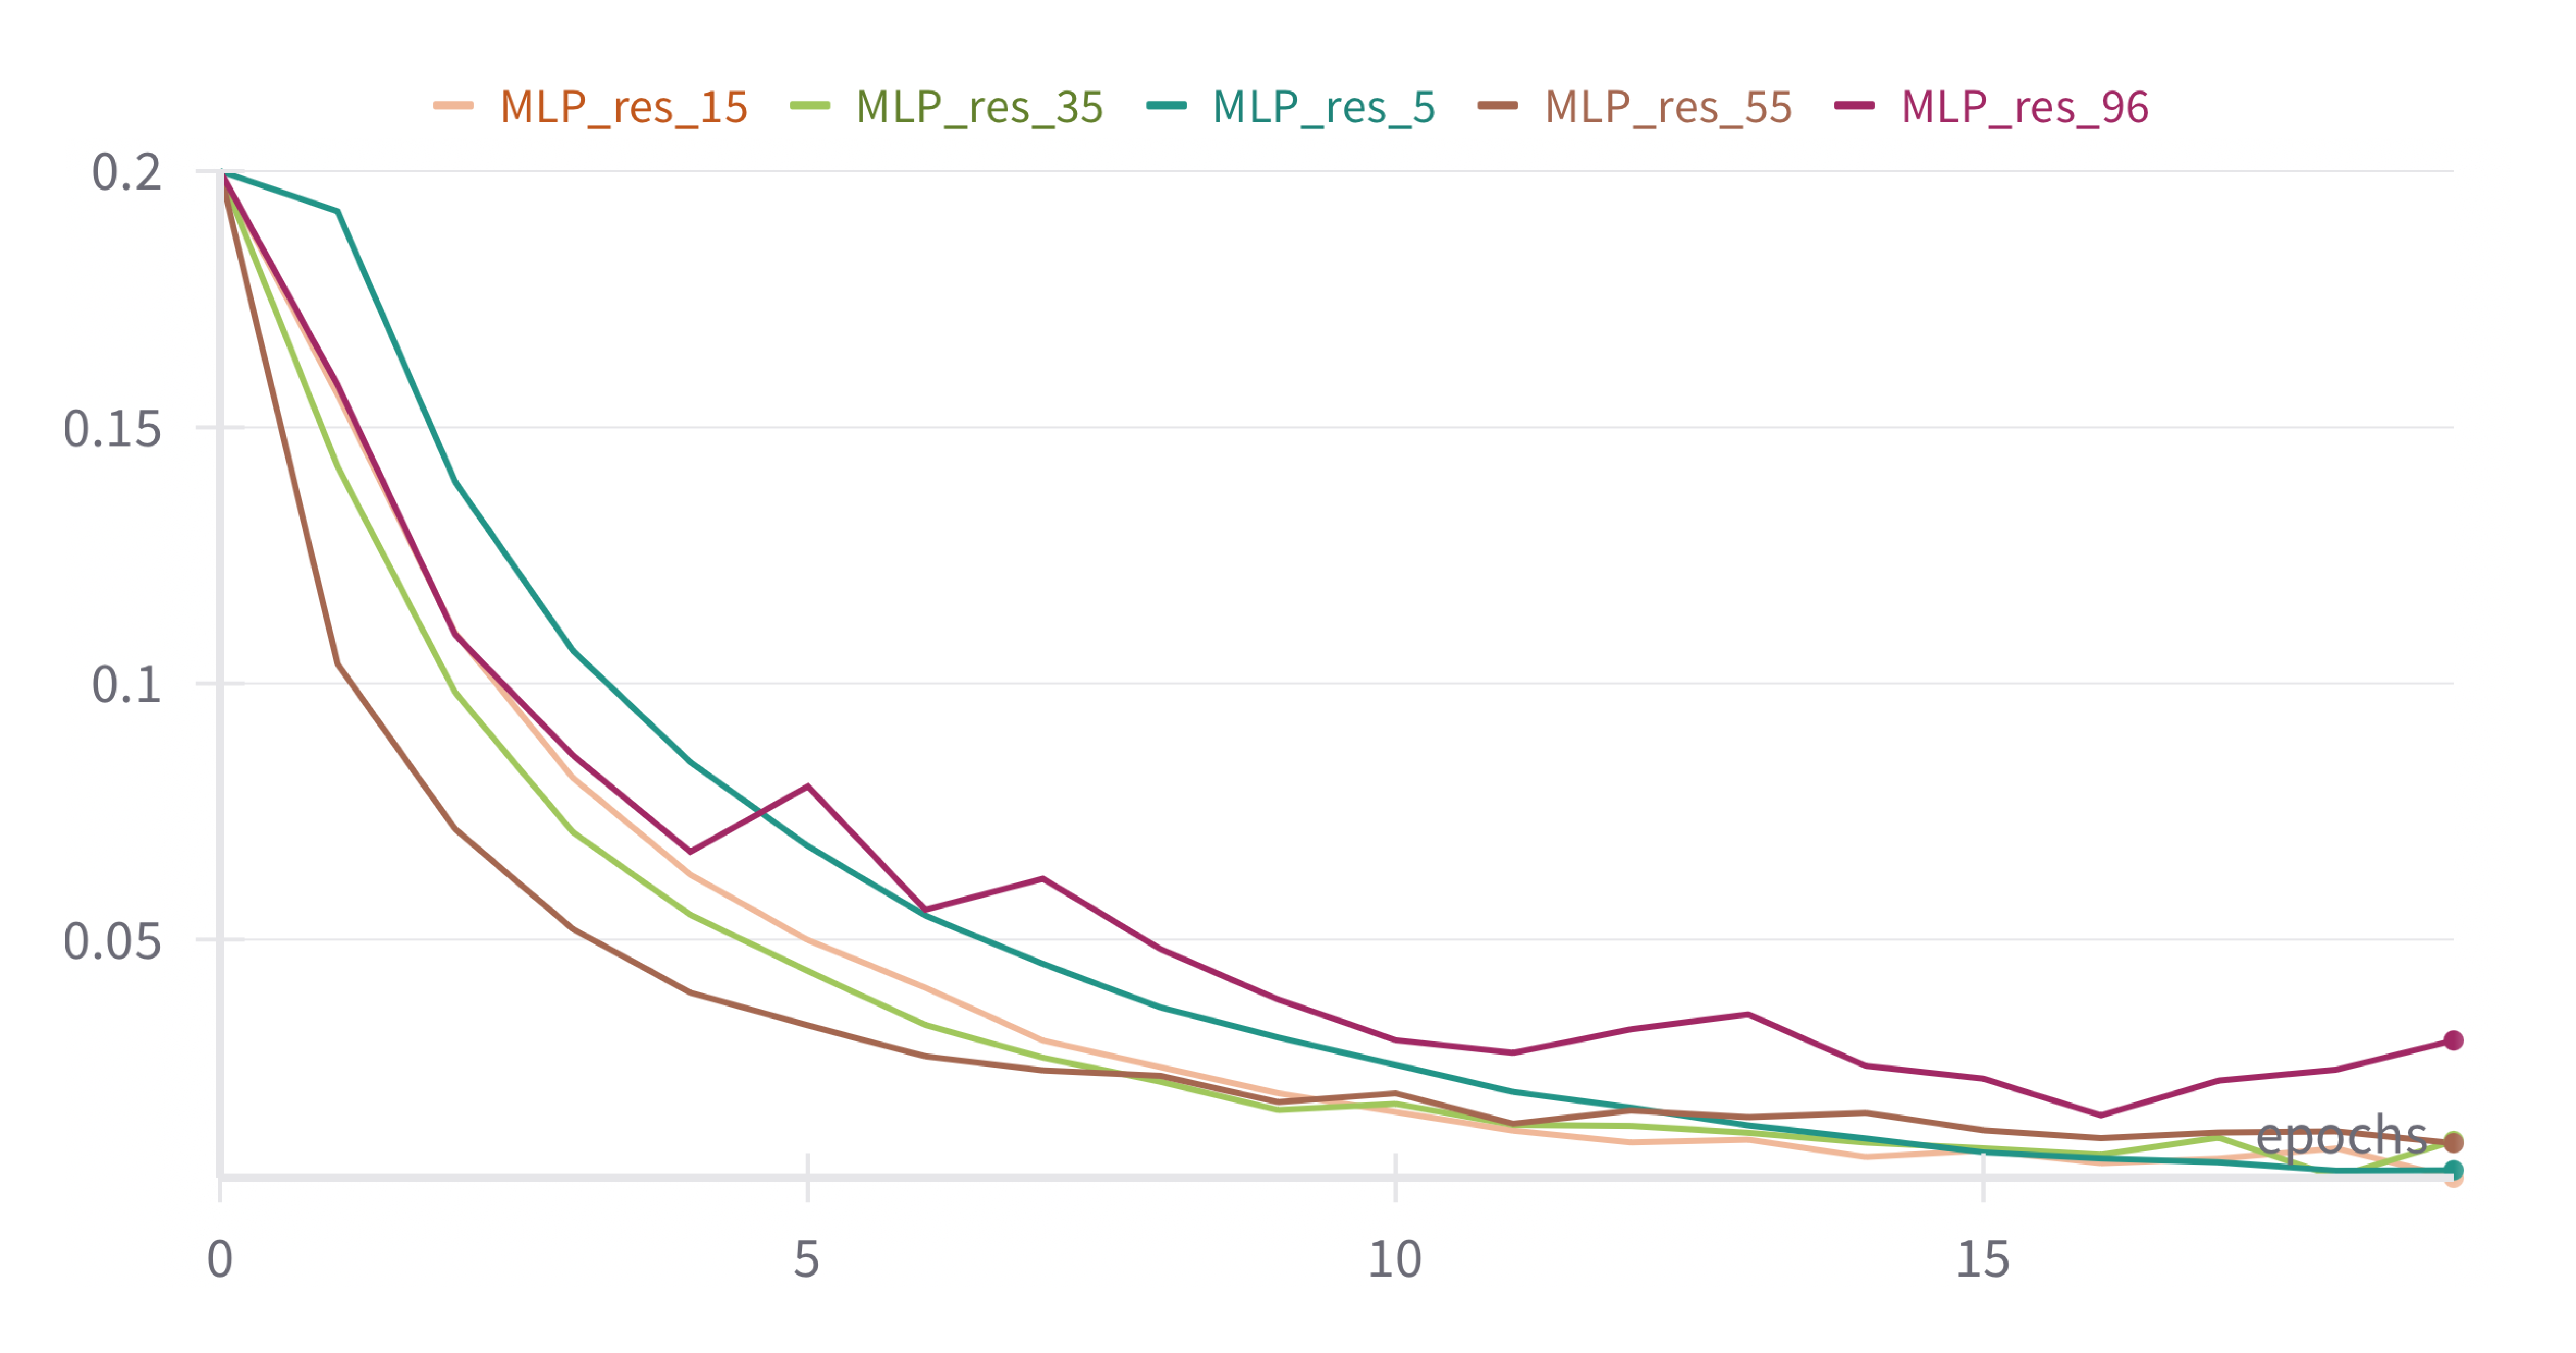
\includegraphics[width=\textwidth]{immages/3-MLP/loss res.pdf}
        \caption{Loss}
    \end{subfigure}
    \hfill
    \begin{subfigure}{0.45\textwidth}
        \centering
        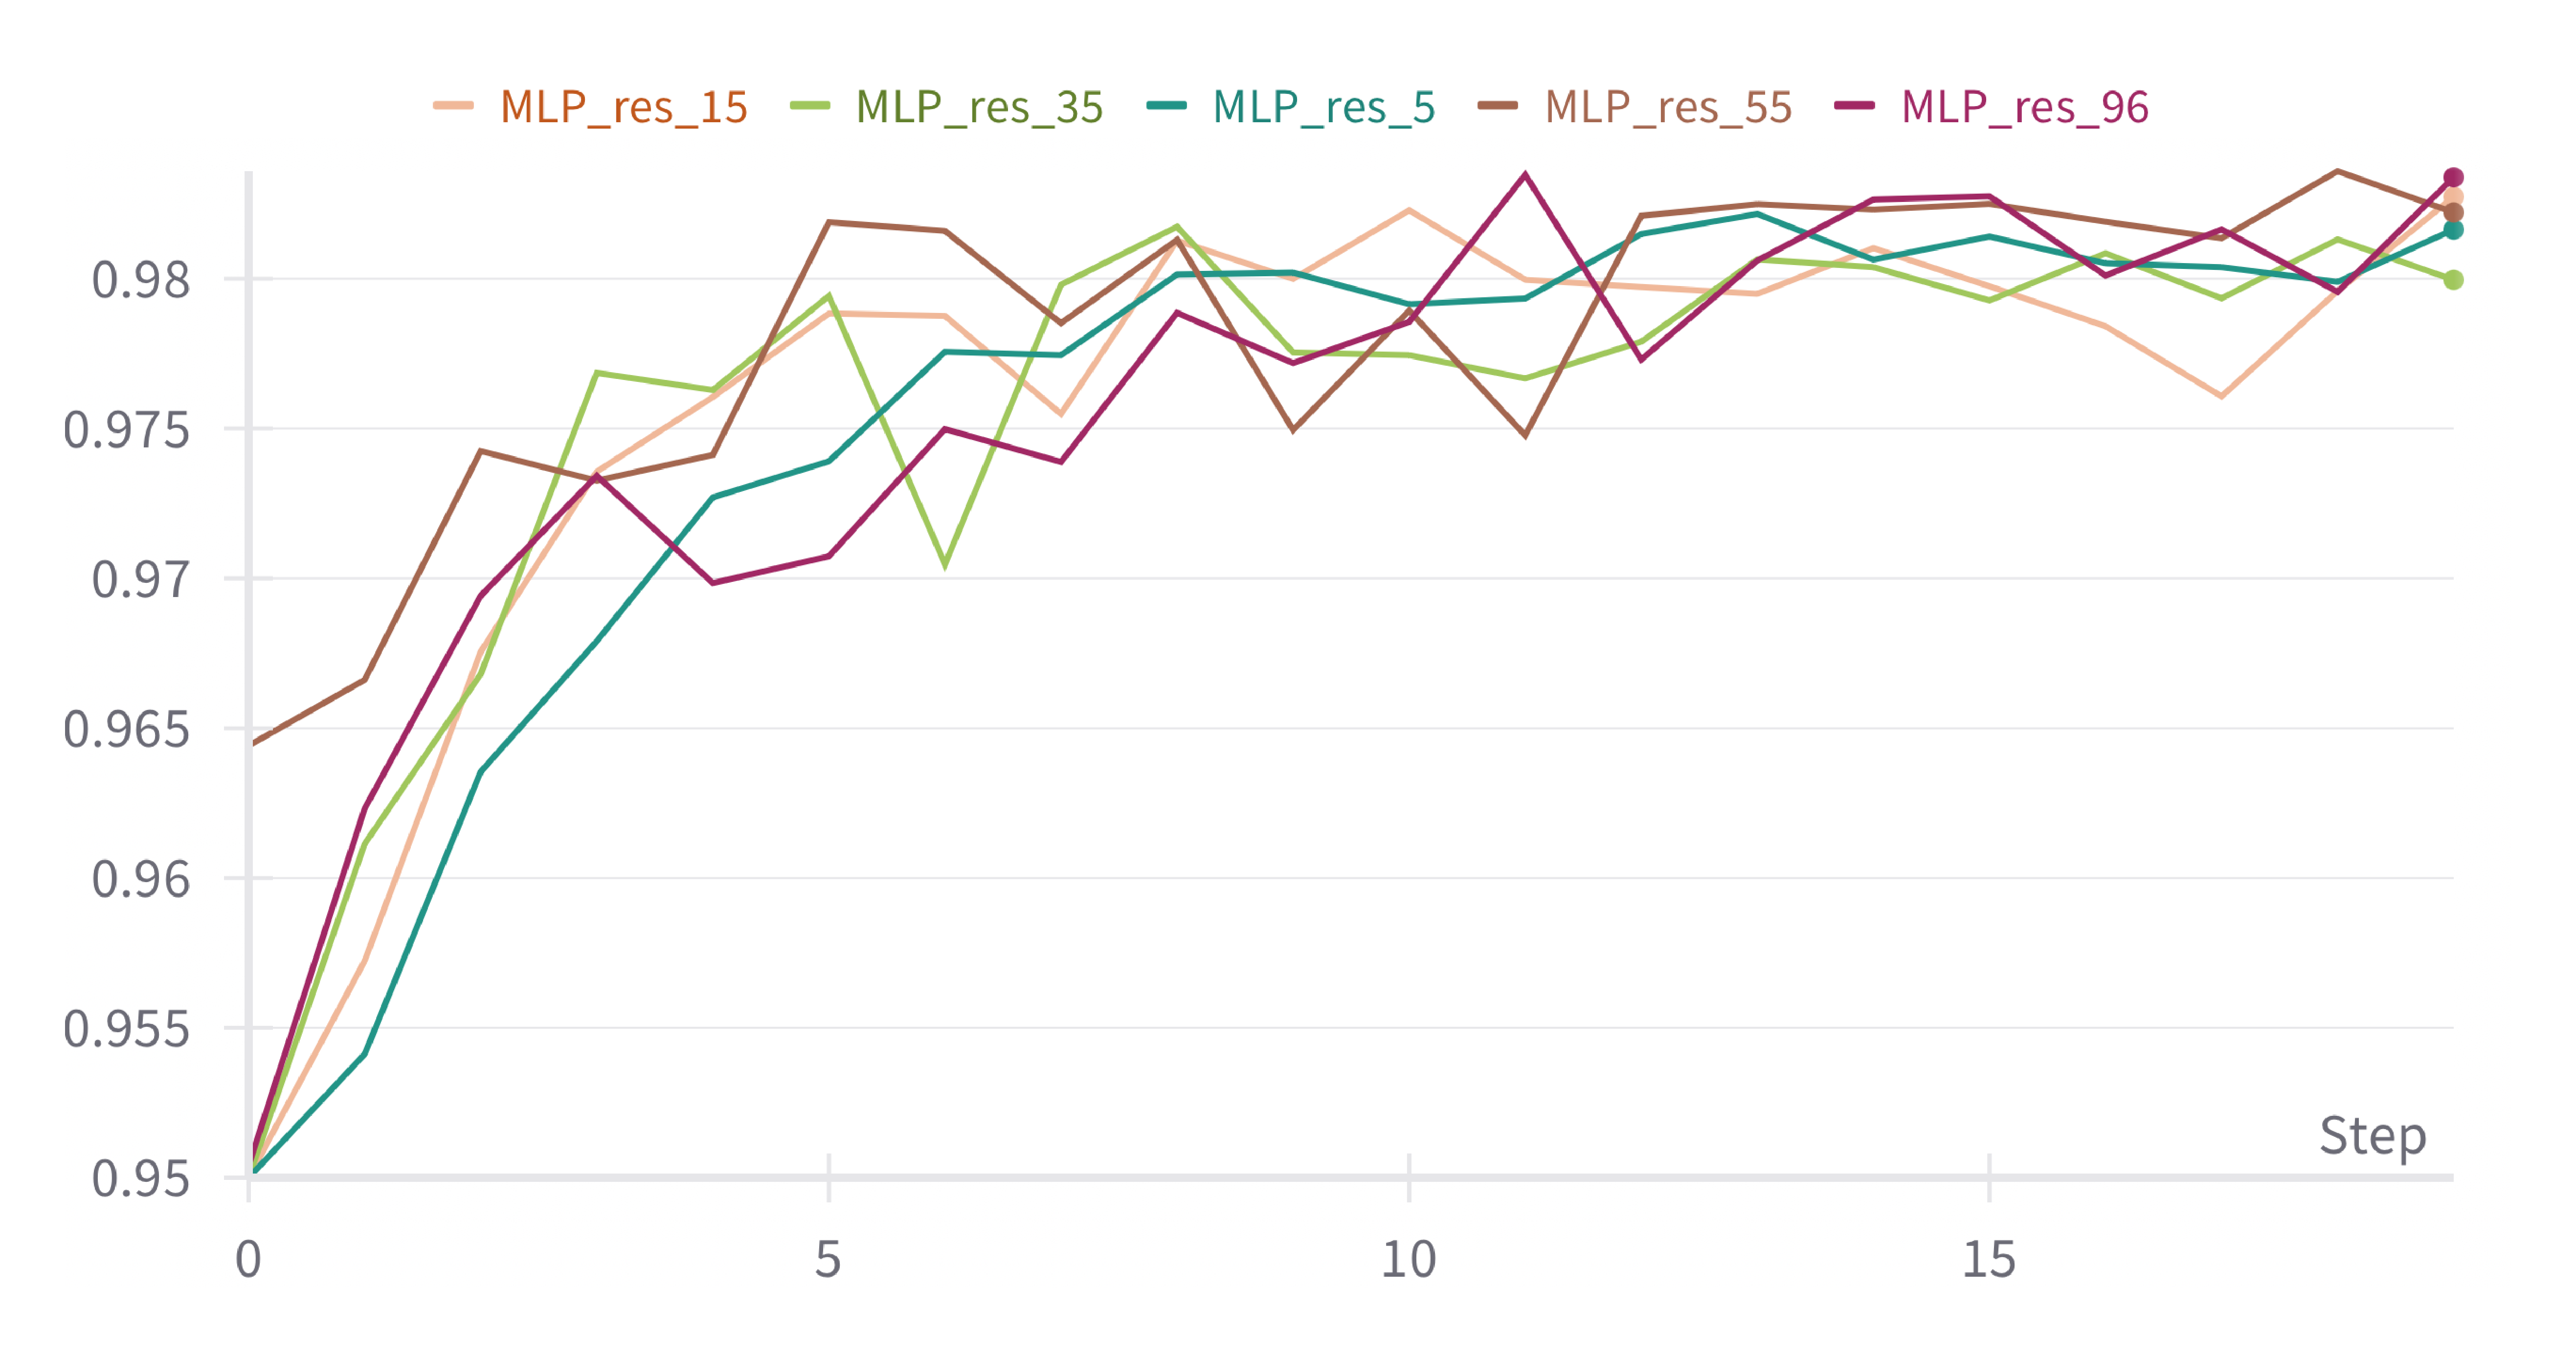
\includegraphics[width=\textwidth]{immages/3-MLP/acc res.pdf}
        \caption{Accuracy}
    \end{subfigure}
    \caption{Loss e Accuracy MLP\_res.}
    \label{fig:MLPres}
\end{figure}

\myskip

Ho pensato che i tempi di addestramento a parità di layer potessero essere diversi, a favore dei modelli che usano le residual connection.
Ho ottenuto però un risultato che non conferma questa ipotesi, come mostrato in Figura \ref{fig:MLPtime}. Questo però potrebbe anche essere dovuto alla semplicità del modello e alla loro (anche se piccola) differenza nel numero di layer. Per questo motivo sarà fatta la stessa analisi su modelli più profondi e complessi nel prossimo capitolo.

\begin{figure}[htbp]
    \centering
    \begin{subfigure}{0.45\textwidth}
        \centering
        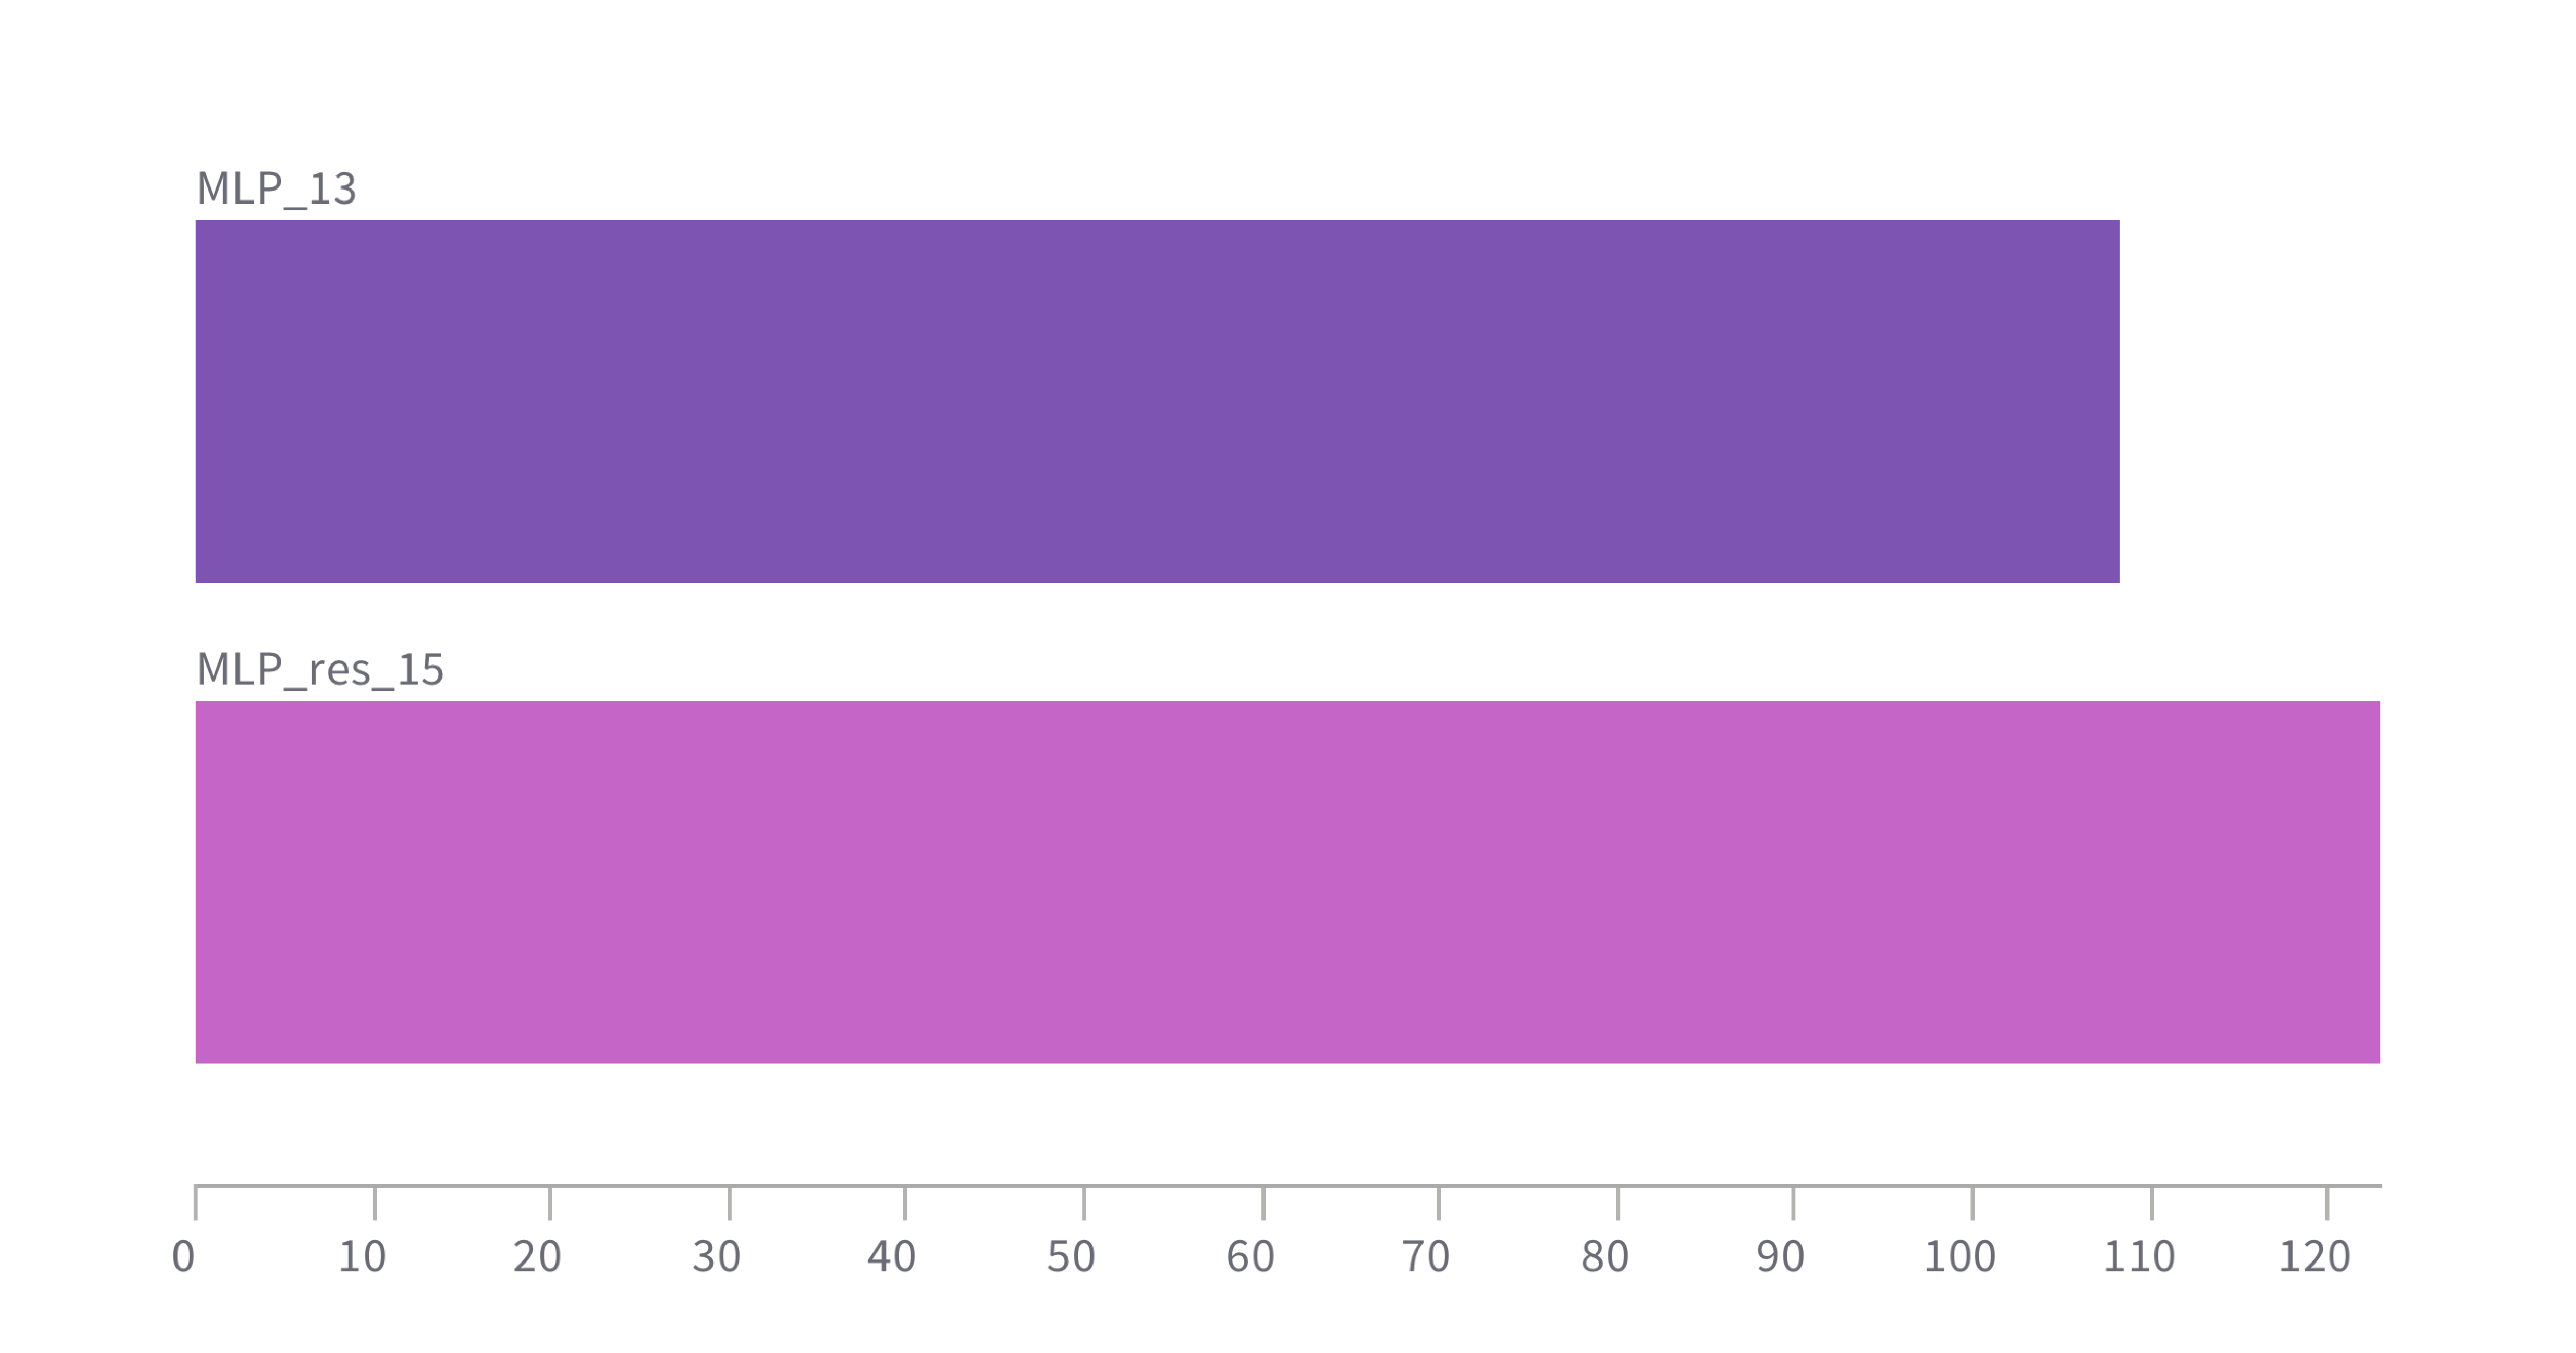
\includegraphics[width=\textwidth]{immages/3-MLP/timeShallow.pdf}
        \caption{Shallow MLP}
    \end{subfigure}
    \hfill
    \begin{subfigure}{0.45\textwidth}
        \centering
        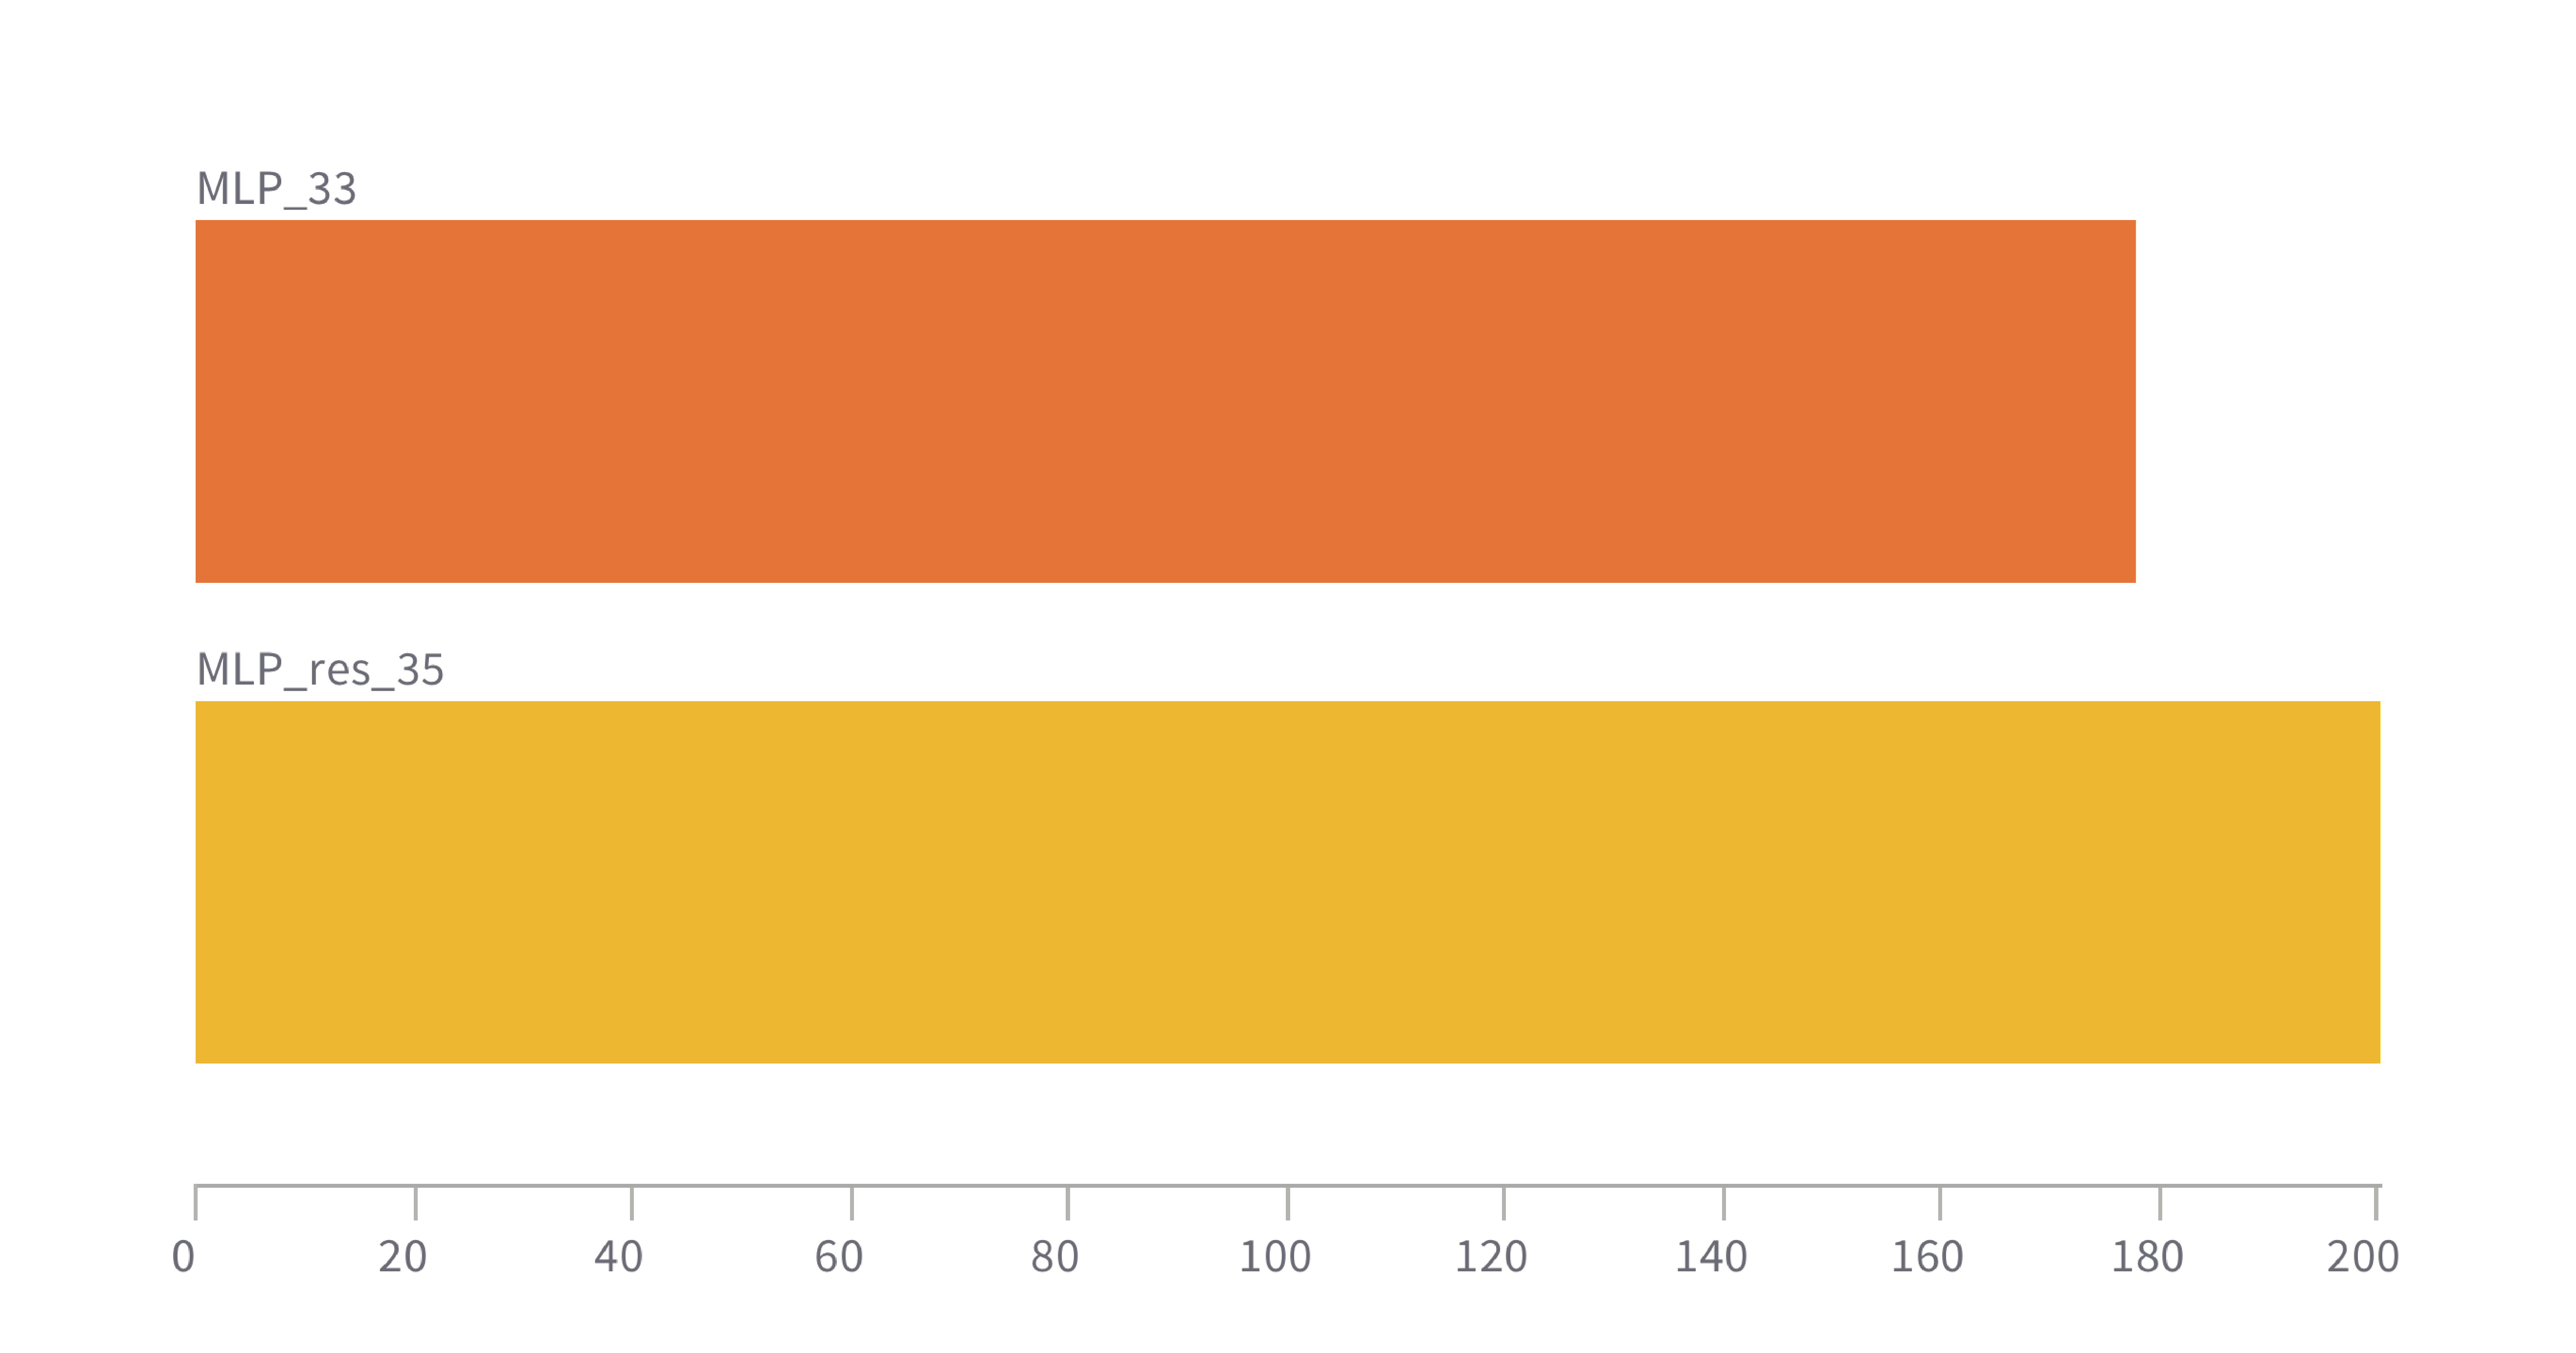
\includegraphics[width=\textwidth]{immages/3-MLP/timeDeep.pdf}
        \caption{Deep MLP}
    \end{subfigure}
    \caption{Training time in second (s).}
    \label{fig:MLPtime}
\end{figure}

\myskip

L'utilità delle residual connection si vede chiaramente anche sulle osservazioni che possiamo fare sui gradienti dei parametri. Se osserviamo infatti la Figura \ref{fig:gradres} vediamo una situazione totalmente diversa rispetto ai modelli senza residual connection: andare in profondità cambia di poco la somma delle norme dei gradienti.

\begin{figure}[htbp]
    \centering
    \includegraphics[width=0.6\textwidth]{immages/3-MLP/grad res.pdf}
    \caption{Somma delle norme dei parametri nei modelli con residual connection.}
    \label{fig:gradres}
\end{figure}